%!TEX root = ../main.tex

\section{The finite-difference scheme}
\label{sec:differential_scheme}

In this section, we present a finite-difference scheme for solving
the equation~\eqref{eq:one_dim} in the domain~$[0, W]_x \times [0,
+\infty)_t$. The equation is
subjected to initial conditions~\eqref{eq:one_dim_initial} and boundary conditions~\eqref{eq:one_dim_marginal}.

Consider a regular mesh with a time step~$\tau$ and
spatial step~$h$. Let~$W = Nh$ with $N$ being the number of
nodes. The nodes of the spatiotemporal grid are given by~$(jh, k \tau)$,
$j = \overline{0, N}$, $k \in \Natural_0$. Define by~$\phi_j^k$
the value of a mesh function~$\phi$ at the node~$(jh, k \tau)$.
Then the finite-difference approximations read
\begin{equation}
  \cfrac{1}{m} \difftau{\phi} = \half K_\phi^2 \epsilon'(\phi_j^k) + \cfrac{\Gamma}{l^2} f'(\phi_j^k) + \cfrac{\Gamma}{2} \diffhh{\phi} \tpoint
  \label{eq:subtractive}
\end{equation}
or, in the explicit form,
\begin{gather}
  \begin{aligned}
    \phi_j^{k + 1} = \phi_j^k + m \tau \left( \half K_\Phi^2 \epsilon'(\phi_j^k) + \cfrac{\Gamma}{l^2} f'(\phi_j^k) + \cfrac{\Gamma}{2} \diffhh{\phi} \right), \\ j = \overline{1, N - 1}, \quad k \in \Natural_0 \tsemicolon
  \end{aligned}
  \label{sch:transition} \\
  \phi_j^0 = \phi_0(jh); \quad \phi_0^k = \phi_l(k \tau); \quad \phi_N^k = \phi_r(k \tau) \tpoint
  \label{sch:borders}
\end{gather}

It is easy to see that the scheme has the first order of approximation in
time and the second order of approximation in spatial terms.

To study properties of the scheme~\eqref{sch:transition}, \eqref{sch:borders},
the linear theory can be used (see, e.g.,
\cite[Chapter~10]{bahvalov_computational_methods}
or~\cite[Chapter~IX]{kalitkin_computational_methods}).
The central result of the theory states, in a somewhat simplified
form, that if a finite-difference scheme is stable and approximates a
continuous problem then the solution of the finite-dimensional problem
converges to the solution of the continuous one with order
not lower then the order of approximation.

To apply this result for the nonlinear setting~\eqref{sch:transition}, \eqref{sch:borders},
we proceed as follows:
(i) linearize the equation~\eqref{eq:subtractive}
for a fixed~$\phi$ and then (ii) apply the spectral stability
argument~\cite{bahvalov_computational_methods} to the
derived linearized equation. As the stability criteria are
satisfied for the linearized equation, stability should be expected for the
complete, nonlinear, problem. In this case, convergence of the
approximate solution should be expected as well~--- since
the finite-difference problem is stable and approximates the continuous
one.
The results of such non-rigorous analysis will be further confirmed by
numerical computations in the fully nonlinear setting.


\subsection{Stability estimate}

In this section we derive a stability condition for the
finite-difference scheme~\eqref{sch:transition}, \eqref{sch:borders}
using the so-called principal of ``frozen coefficients''
(see, e.g.,~\cite{bahvalov_computational_methods}).
Let~$\phi_j^k$ and~$\phi_j^k + \delta_j^k$ be solutions of the
finite-difference equation~\eqref{eq:subtractive}.
Substitute~$\phi_j^k + \delta_j^k$ into~\eqref{eq:subtractive} to obtain:
\begin{multline*}
  \cfrac{1}{m} \cfrac{(\phi_j^{k + 1} + \delta_j^{k + 1}) - (\phi_j^k + \delta_j^k)}{\tau} = \half K_\Phi^2 [\epsilon'(\phi_j^k) + \epsilon''(\phi_j^k) \delta_j^k + o(\delta_j^k)] + \\ + \cfrac{\Gamma}{l^2} [f'(\phi_j^k) + f''(\phi_j^k) \delta_j^k + o(\delta_j^k)] + \cfrac{\Gamma}{2} \cfrac{(\phi_{j + 1}^k + \delta_{j + 1}^k) - 2 (\phi_j^k + \delta_j^k) + (\phi_{j - 1}^k + \delta_{j - 1}^k)}{h^2} \tpoint
\end{multline*}
Linearizing this equation around~ $\phi_j^k = P$, assuming that
perturbations~$\delta_j^k$ are small and taking into account
that~$\phi_j^k$ is a solution of the finite-difference problem, we obtain:
\begin{equation}
  \delta_j^{k + 1} = \delta_j^k + m \tau \left( \half K_\Phi^2 \epsilon''(P) \delta_j^k + \cfrac{\Gamma}{l^2} f''(P) \delta_j^k + \cfrac{\Gamma}{2} \diffhh{\delta} \right) \tpoint
  \label{eq:scheme_variation}
\end{equation} 

We now apply spectral stability analysis to the derived equation for
perturbations.
Let~$\delta_j^k = \lambda(\theta)^k \cdot \exp(\imath j \theta)$, $\imath^2 = -1$.
Substituting this representation into~\eqref{eq:scheme_variation} one obtains:
$$\lambda(\theta) = 1 + m \tau \left( \half K_\Phi^2 \epsilon''(P) + \cfrac{\Gamma}{l^2} f''(P) + \cfrac{\Gamma}{2} \cfrac{\exp(\imath \theta) - 2 + \exp(-\imath \theta)}{h^2} \right) \tcomma$$
or
\begin{equation}
  \lambda(\theta) = 1 + m \tau \left( \half K_\Phi^2 \epsilon''(P) + \cfrac{\Gamma}{l^2} f''(P) - \cfrac{2 \Gamma}{h^2} \sin^2 \cfrac{\theta}{2} \right) \tpoint
  \label{eq:spectral}
\end{equation}

According to the spectral stability argument, a time
step~$\tau = \tau(h)$ provides stability of the scheme in the
domain~$[0, W]_x \times [0, T]_t$ with~$T<+\infty$ as~$\tau, h \to 0$ if there
exists~$C > 0$ such that for an arbitrary~$\theta$ it
holds~$|\lambda(\theta)| \leqslant \exp(C\tau)$. Note that here it is
also possible to use more strict condition~$|\lambda(\theta)| \leqslant 1 + C\tau$.
If for an arbitrary~$\theta$ it holds~$|\lambda(\theta)| \leqslant 1$,
then stability will be provided also for an unbounded time interval, i.e.,
for~$[0, W]_x \times [0, +\infty)_t$.
Strictly speaking, the spectral argument does not provide a sufficient
stability condition; however, stability should be expected in practice.

First, consider the expression~\eqref{eq:spectral} for~$P=0$.
We have~$f''(0) = 0$, $\epsilon''(0) = 0$, and the equation~\eqref{eq:spectral}
takes the form of
$$\lambda(\theta) = 1 - \cfrac{2 \tau m \Gamma}{h^2} \sin^2 \cfrac{\theta}{2} \tpoint$$
Hence, for an arbitrary~$\theta$ it holds~$|\lambda(\theta)| \leqslant 1$
if and only if
\begin{equation}
  \tau \leqslant \cfrac{h^2}{m \Gamma} \tpoint
  \label{cond:spectral_0}
\end{equation}
As the condition~\eqref{cond:spectral_0} is satisfied, one can expect stability of the scheme
when the solution describes an almost completely damaged state~$\phi\approx0$
in the domain~$[0, W]_x \times [0, +\infty)_t$.

Note that under the condition~\eqref{cond:spectral_0} one also can expect stable computations
for~$[0, W]_x \times [0, T]_t$ for an arbitrary value~$P \in [0, 1]$.
In this case the following is true:
$$
|\lambda(\theta)| \leqslant \left| 1 - \cfrac{2 \tau m \Gamma}{h^2} \sin^2 \cfrac{\theta}{2} \right| + m \tau \left| \half K_\Phi^2 \epsilon''(P) + \cfrac{\Gamma}{l^2} f''(P) \right| \leqslant 1 + m \tau \left| \half K_\Phi^2 \epsilon''(P) + \cfrac{\Gamma}{l^2} f''(P) \right| \tpoint
$$
Hence, there exists~$C$ such that
$|\lambda(\theta)| \leqslant 1 + C \tau$ holds,~--- since~$\epsilon''(\phi)$ and~$f''(\phi)$
are continuous on~$[0, 1]$.
It should be noted that, despite such versatility, the estimate~\eqref{cond:spectral_0}
is poorly applicable in practice and requires clarification, which will be done later.

We now consider the expression~\eqref{eq:spectral} at the value~$P=1$.
Note that~$f''(1) < 0$, $\epsilon''(1) > 0$.
We see that for~$(K_\Phi^2 / 2) \epsilon''(1) + (\Gamma / l^2) f''(1) \leqslant 0$
it is possible to achieve~$|\lambda(\theta)| \leqslant 1$ with demanded sufficiently small
values of~$\tau$ and the condition $\tau \leqslant h^2 / (2m \Gamma)$,
similar to the one for~\eqref{cond:spectral_0}.
Substituting~$f''(1) = -12, \; \epsilon''(1) = 12 \epsilon_0 / (1 + \delta)^2$
(see~\eqref{eq:epsilon_derivatives}),
we obtain
\begin{equation}
  \cfrac{K_\Phi^2 l^2 \epsilon_0}{2 \Gamma (1 + \delta)^2} \leqslant 1 \tpoint
  \label{cond:spectral_possible_1}
\end{equation}

So, under the condition~\eqref{cond:spectral_possible_1}, it is expected that
there exist such values of~$\tau$ и $h$
that the difference scheme is stable for~$\phi \approx 1$
and~$T=+\infty$.
Naturally the condition~\eqref{cond:spectral_possible_1}
is equivalent to the stability condition~\eqref{cond:equilibrium_1_stable}
for the equilibrium state~$\phi \equiv 1$ of the equation~\eqref{eq:one_dim}.

\subsection{Improved stability estimate}

In the previous section form the analysis of equation~\eqref{eq:spectral}
it was derived stability condition~\eqref{cond:spectral_0}
for finite-difference scheme~\eqref{sch:transition} and~\eqref{sch:borders} for~$\phi \approx 0$.
The assumption of its usefulness is based on the fact that typical ``'natural'' solution of the model
will has a form of the transition process from the undamaged state~$\phi=1$ to the completely
damaged state~$\phi=0$ occurring in a finite time interval and then infinitely long staying in the
damaged state~$\phi \approx 0$.


However the performed analysis of the equation~\eqref{eq:spectral}
is not sufficient at~$\phi = 0$. Indeed, it was used that at~$\phi=0$,
$\epsilon''(0) = 0$ (see expression~\eqref{eq:epsilon_derivatives}),~---
but it was not accounted that~$\epsilon''(\phi)$ growth fast and reaches
large values  for small values of~$\delta\approx 0$,
see Fig.~\ref{fig:eps_phi_phi}.
This means that the equations of the model are stable at~$\phi=0$,
but can be unstable in the small neighbourhood of~$\phi=0$.
Such situation is not satisfactory and we now try to improve
the obtained stability estimates.
%
\begin{figure}[!t]
	\centering
	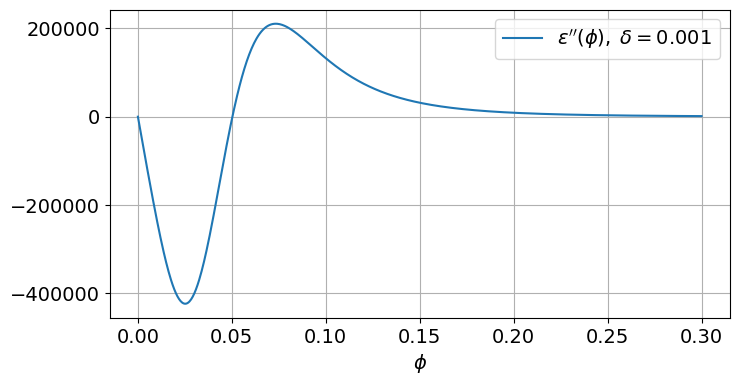
\includegraphics[width=\textwidth]{figures/eps_phi_phi.png}
	\vspace{-0.7cm}
	\caption{Typical behavior of~$\epsilon''(\phi)$ in the vicinity of~$0$.}
	\label{fig:eps_phi_phi}
\end{figure}

To proceed let us estimate extremums of~$\epsilon''(\phi)$ in the neighbourhood of~$0$.
First, find zeros of~$\epsilon'''(\phi)$. We have
\begin{equation}
	\epsilon''' = \epsilon_0 \cfrac{-6 (f')^3 + 6 (f + \delta) f' f'' - (f + \delta)^2 f'''}{(f + \delta)^4},
	\label{eq:epsilon_phi_phi_phi}
\end{equation}
form where:
$$\epsilon'''(\phi) = -6 (f')^3 + 6 (f + \delta) f' f'' - (f + \delta)^2 f''' = 0 \tcomma$$
or, taking~\eqref{eq:epsilon} into account:
$$-3 \cdot 12^2 (1 - \phi)^3 + 36 \left(4 - 3\phi + \cfrac{\delta}{\phi^3} \right)(1 - \phi)(2 - 3\phi) - \left(4 - 3 \phi + \cfrac{\delta}{\phi^3} \right)^2 (1 - 3 \phi) = 0 \tpoint$$

Let~$\delta_n \to +0$ and~$\phi_n \to +0$ such that~$\delta_n / \phi_n^3$ is bounded.
Then:
\begin{gather*}
	-3 \cdot 12^2 \cdot 1^3 + 36 \left(4 + \cfrac{\delta_n}{\phi_n^3} \right) \cdot 1 \cdot 2 - \left(4 + \cfrac{\delta_n}{\phi_n^3} \right)^2 \cdot 1 \to 0 \tcomma \\
	\left(4 + \cfrac{\delta_n}{\phi_n^3} \right)^2 - 72 \left(4 + \cfrac{\delta_n}{\phi_n^3} \right) + 3 \cdot 12^2 \to 0 \tpoint
\end{gather*}
Hence, a sequence~$4 + \delta_n / \phi_n^3$ has not more than two partial limits~$\xi_+$ and~$\xi_-$~---
which are zeros of the equation~$\xi^2 - 72 \xi + 432 = 0$.
To the first zero~$\xi_+ = 36 + 12 \sqrt{6}$ it corresponds
$$\phi_+ = \cfrac{1}{\sqrt[3]{32 + 12 \sqrt{6}}} \sqrt[3]{\delta_n} \approx \cfrac{1}{3.945} \sqrt[3]{\delta_n} \tsemicolon$$
to the second zero~$\xi_- = 36 - 12 \sqrt{6}$ it corresponds
$$\phi_- = \cfrac{1}{\sqrt[3]{32 - 12 \sqrt{6}}} \sqrt[3]{\delta_n} \approx \cfrac{1}{1.376} \sqrt[3]{\delta_n} \tpoint$$

From here it can be seen that for~$\delta \to +0$ the function~$\epsilon'''(\phi)$ has two zeros in the neighbourhood of~$0$:
\begin{equation}
  \phi_{\pm} = \cfrac{1}{\sqrt[3]{32 \pm 12 \sqrt{6}}} \sqrt[3]{\delta} [1 + o(1)] \tpoint
  \label{eq:epsilon_phi_phi_phi_roots}
\end{equation}

We now estimate~$\epsilon''(\phi)$ at~$\phi_{\pm}$  for~$\delta \to +0$. Let~$\phi = (1 / c) \sqrt[3]{\delta}$, $c \in \Real$.
Then:
$$\epsilon'' = \epsilon_0 \cfrac{24 c^5 (8 - c^3)}{(4 + c^3)^3} \delta^{-5 / 3} [1 + o(1)],$$
and:
\begin{equation}
  \epsilon''(\phi_+) \approx -4.378 \epsilon_0 \delta^{-5 / 3}; \quad \epsilon''(\phi_-) \approx 2.216 \epsilon_0 \delta^{-5 / 3} \tpoint
  \label{est:epsilon_phi_phi_bounds}
\end{equation}
The derived estimates are shown as black dashed lines on Fig.~\ref{fig:eps_phi_phi_multiplied}.

\begin{figure}[!t]
	\centering
	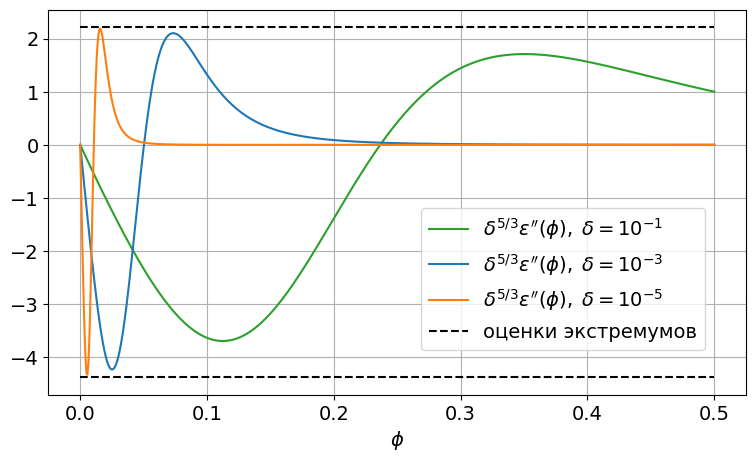
\includegraphics[width=\textwidth]{figures/eps_phi_phi_multiplied.png}
	\caption{Qualitative behavior of~$\delta^{5 / 3} \epsilon''(\phi)$ for small values of~$\delta$.}
	\label{fig:eps_phi_phi_multiplied}
\end{figure}

Now, to derive new stability estimate we consider equation~\eqref{eq:spectral} at~$\phi = \phi_+$.
Note that~$\epsilon''(\phi_+) \approx -4.4 \epsilon_0 \delta^{-5 / 3}$.
The term inside braces in~\eqref{eq:spectral} is negative since
$\delta$ is small and~$\epsilon''(\phi_+)$ is negative and large in its absolute value.
Therefore~$f''(\phi_+) > 0$ can be estimated as~$0$~--- such estimate makes inequality stronger.
Then from inequality~\eqref{eq:spectral} it follows that 
$$\lambda(\theta) = 1 + m \tau \left( -\cfrac{2.2 K_\Phi^2 \epsilon_0}{\delta^{5 / 3}} - \cfrac{2 \Gamma}{h^2} \sin^2 \cfrac{\theta}{2} \right) \tpoint$$
Condition~$|\lambda(\theta)| \leqslant 1$ is satisfied for an arbitrary~$\theta$, if and only if
\begin{equation}
  \tau \leqslant \cfrac{1}{m} \left( \cfrac{1.1 K_\Phi^2 \epsilon_0}{\delta^{5 / 3}} + \cfrac{\Gamma}{h^2} \right)^{-1} \tpoint
  \label{cond:spectral_better_theoretical}
\end{equation}

Numerical experiments described in the next sections indicates that
more strong version of the estimate~\eqref{cond:spectral_better_theoretical} is also valid
(note the doubled denominator):
%
\begin{equation}
  \tau \leqslant \cfrac{1}{2m} \left( \cfrac{K_\Phi^2 \epsilon_0}{\delta^{5 / 3}} + \cfrac{\Gamma}{h^2} \right)^{-1} \tpoint
  \label{cond:spectral_better}
\end{equation}

Finally, more simple estimate not weaker then~\eqref{cond:spectral_better} is:
\begin{equation}
  \tau \leqslant \cfrac{1}{4m} \min \left(\cfrac{\delta^{5 / 3}}{K_\Phi^2 \epsilon_0}, \; \cfrac{h^2}{\Gamma} \right) \tpoint
  \label{cond:spectral_better_simpler}
\end{equation}

Note that the derived stability estimate~\eqref{cond:spectral_better}
for finite-difference scheme~\eqref{sch:transition},\eqref{sch:borders}
includes all the parameters of the equation~\eqref{eq:one_dim}, except~$l$.
Notably, this is the only parameter of the model which has somehow artificial nature and can not be
related directly to the underlying physics.

\endinput
% EOF